
\documentclass[a4paper, oneside, 11pt]{report}
\usepackage{epsfig,pifont,float,multirow,amsmath,amssymb}
\newcommand{\mc}{\multicolumn{1}{c|}}
\newcommand{\mb}{\mathbf}
\newcommand{\mi}{\mathit}
\newcommand{\oa}{\overrightarrow}
\newcommand{\bs}{\boldsymbol}
\newcommand{\ra}{\rightarrow}
\newcommand{\la}{\leftarrow}
%\usepackage{algorithm}
%\usepackage{algorithmic}
\topmargin = 0pt
\voffset = -80pt
\oddsidemargin = 15pt
\textwidth = 425pt
\textheight = 750pt

\begin{document}

\begin{titlepage}
\begin{center}
\rule{12cm}{1mm} \\
\vspace{1cm}
{\large  CMP-6048A Advanced Programming} %Delete as appropriate
\vspace{7.5cm}
\\{\Large Project Report - 13 January 2025}
\vspace{1.5cm}
\\{\LARGE Maths Interpreter software} % You can add to this title of modify it if you wish
\vspace{1.0cm}
\\{\Large Group members: \\ Connor Stansfield, Ethan Colman, Taylor Holton, Aaron Hurrell\ }
\vspace{10.0cm}
\\{\large School of Computing Sciences, University of East Anglia}
\\ \rule{12cm}{0.5mm}
\\ \hspace{8.5cm} {\large Version 2.0}
\end{center}
\end{titlepage}


\setcounter{page}{1}
%\pagenumbering{roman}
%\newpage


\begin{abstract}
Please replace this section with your own abstract. An abstract is a brief summary (maximum 250 words) of your entire project. It should cover your objectives, your methodologies used, a brief developmental history, your final results, in particular covering the optional tasks, and a discussion and conclusion. You do not cover the literature or background in an abstract nor should you use abbreviations or acronyms. The remainder of this report template has clear chapter titles and we suggest to stick to these although you can organise your material inside each chapter to your own preferences. A guideline in size is approximately 3,500 words (not including abstract, captions and references) but no real limit on figures, tables, diagrams, pseudo-code etc.
\end{abstract}

\chapter{Introduction}
\label{chap:intro}

The introduction should be brief and comprise the following:

\section{Project statement}
A (brief) statement including the nature of the project, i.e.\ what you will do, how you will accomplish it and what the final deliverable will be.

\section{Aims and objectives}

Clearly specify the main aim and objective(s) and subsequent tasks of your project. You can use a MoSCoW to further elaborate on each individual task. If you do so, use a table with three columns (e.g.\ Table \ref{Table1}), the first one having the four categories; the second column a brief description of the task and the third column further elaboration or comments on the task. Note that a MoSCoW is normally for functional requirements only. You should treat non-functional requirements in a separate MoSCoW.

\begin{table}[h]
\caption{MoSCoW}
\begin{center}
\begin{tabular}{|p{1in}|p{2in}|p{2.5in}|} \hline
Priority & Task & Comments \\ \hline \hline
\multirow{3}{1in}{Must}
& Task M1 & Comment M1 \\ \cline{2-3}
& Task M2 & Comment M2 \\ \cline{2-3}
& ... & ... \\ \hline \hline
\multirow{3}{1in}{Should}
& Task S1 & Comment S1 \\ \cline{2-3}
& Task S2 & Comment S2 \\ \cline{2-3}
& ... & ... \\ \hline \hline
\multirow{3}{1in}{Could}
& Task C1 & Comment C1 \\ \cline{2-3}
& Task C2 & Comment C2 \\ \cline{2-3}
& ... & ... \\ \hline \hline
\multirow{3}{1in}{Should not}
& Task SN1 & Comment SN1 \\ \cline{2-3}
& ... & ... \\ \hline
\end{tabular}
\label{Table1}
\end{center}
\end{table}


\chapter{Background}

Give a brief background on similar software, e.g.\ \cite{Desmos:2023}, \cite{Matlab:2023}, etc.
Also cite the books \cite{Nystrom:2021} or documentation \cite{WPF:2023} that you consulted.
You should add additional references to the corresponding bib file (References.bib) referred to in the bottom of this document.


\chapter{Development History}\label{Chap:DevHist}

Describe the history of your development in terms of the iterations or sprints in your project (your Github repository or other version control should help you to retrospectively identify these). Use different sections for different sprints and subsections for specific details on the same sprint. Feel free to use subsubsections or paragraphs (which are not numbered) if needed. 

\section{Sprint 1: Basic expressions and GUI}
\subsection{Grammar in BNF}
\begin{verbatim}
<E>    ::= <T> <Eopt>
<Eopt> ::= "+" <T> <Eopt> | "-" <T> <Eopt> | <empty>
<T>    ::= <NR> <Topt>
<Topt> ::= "*" <NR> <Topt> | "/" <NR> <Topt> | <empty>
<NR>   ::= "Num" <value> | "(" <E> ")"
\end{verbatim}

\subsection{Basic GUI}
We used WPF with C\# to develop a basic GUI - see Figure \ref{gui01}.

\begin{figure}[htb]
\begin{center}
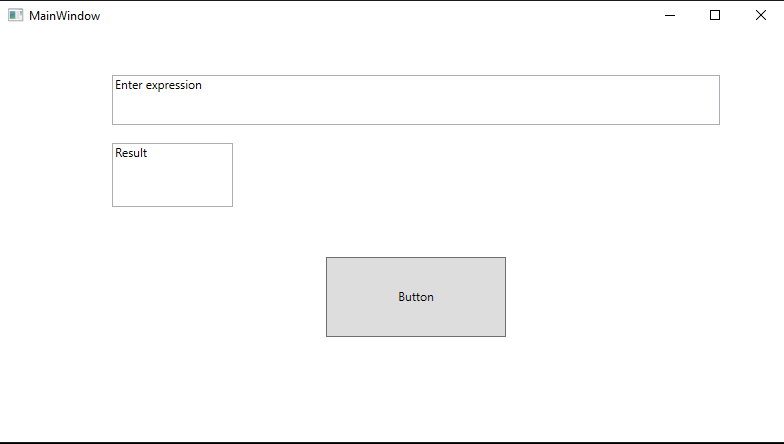
\includegraphics[width=0.9 \columnwidth]{GUI_01.png}
\caption{A very basic GUI!}
\label{gui01}
\end{center}
\end{figure}

\subsection{Testing}
A subset of Table \ref{Table2} in Appendix \ref{app:test} could be referred to from here.

\section{Sprint 2: Adding unary minus, powers and mod}

\subsection{BNF}

\subsection{Updated GUI}

\section{Sprint 3: ...}

\section{Sprint n: Your penultimate version}

Make sure that the total number of sprints n(+1) does not become too unwieldy. A rule of thumb would expect it to be somewhere between 6 and 12.

\subsection{BNF}

\subsection{}

\chapter{Final deliverable}\label{Impl}

In this chapter you cover the final or ``ultimate'' version of your project. It will show the final BNF, the final GUI, the architecture (which should be MVVM or MVC) that includes UML diagrams, additional algorithms if not already included in the previous sprint sections.

\section{Final BNF}

\section{Final GUI}

See Figure \ref{gui02}.

\begin{figure}[htb]
%\begin{center}
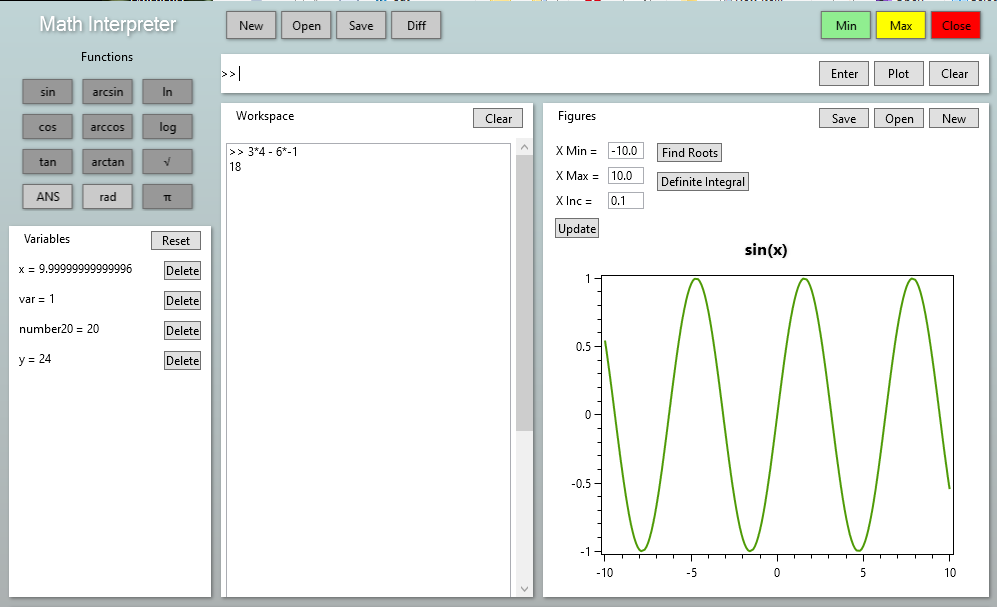
\includegraphics[width=0.9 \columnwidth]{GUI_02.png}
\caption{A potentially final GUI!}
\label{gui02}
%\end{center}
\end{figure}

\section{Code architecture}

Fig.\ \ref{class} shows a UML class diagram (class, sequence and state diagrams are the most frequently used UML diagrams). Illustrating your code architecture - that should be of the MVC family and, considering it is developed in C\# with WPF more specifcally the MVVM pattern - is very important.

\begin{figure}[htb]
%\begin{center}
\includegraphics[width=1.0 \columnwidth]{class.png}
\caption{A UML class diagram to be replaced with yours!}
\label{class}
%\end{center}
\end{figure}

\section{Algorithms}

Algorithms can be described in this chapter if not already covered in previous sections. Pseudo-code is preferred over code snippets. If you use the latter then make sure it is well commented inside the code or via the figure caption. 

\begin{algorithm}[th]
\caption{ The Newton-Raphson method }
%\begin{algorithmic}[1]
\STATE Initialise root based on estimate
\STATE Set stop criterion
\\ \texttt{const double error = 0.000001;}
\WHILE {stop criterion not met}
	\STATE Compute f(root)
	\STATE Compute f'(root)
	\STATE root := root - f(root)/f'(root)
\ENDWHILE
%\end{algorithmic}
\end{algorithm}


Note that code snippets or lists of crucial programming code or large UML diagrams should go in Appendix \ref{app:other} (or further appendices).

\subsection{Testing}

Describe what testing you have done on the interpreter (lexer, parser and execution), GUI and GUI-Interpreter communication, plotting, etc. Table \ref{Table2} in Appendix \ref{app:test} should be completed to do basic arithmetic expression tests.


\chapter{Discussion, conclusion and future work}

Briefly discuss  your achievements and put them in perspective with the MoSCoW analysis you specified in Table \ref{Table1}. Also discuss future developments and how you see the deliverable improving if more time could be spent. Note that this section should not be used as a medium to vent frustrations on whatever did not work out (group issues, not enough time, illness, etc.) as this should be dealt with separately - keep it professional!


\bibliographystyle{apalike}
%\raggedright
\bibliography{References}


\appendix
\chapter{Contributions}

State here the \% contribution to the project of each individual member of the group and describe in brief what each member has done (if this corresponds to particular sections in the report then please specify these).

\chapter{Testing}
\label{app:test}
\section{Arithmetic expression testing}

\begin{table}[h]
\caption{Arithmetic expression tests. Note that floating pointing values are accurate to three decimal places for the fractional part. ResE is expected result and ResA is actual result. \\}
\begin{tabular}{|p{1.8in}|p{0.5in}|p{0.4in}|p{0.6in}|p{1.4in}|} \hline
Expression & ResE & ResA& Pass/Fail & Action/comment \\ \hline \hline
$5*3+(2*3-2)/2+6$ & 23 &  &  &  ... \\ \hline
$9-3-2$ & 4 & & & left assoc.\  \\ \hline
$10/3$ & 3 & & & int division  \\ \hline
$10/3.0$ & 3.333 & & & float division \\ \hline
$10\%3$ & 1 & & & \\ \hline
$10 - -2$ & 12 & & & unary minus\\ \hline
$-2 + 10$ & 8 & & & \\ \hline
$3*5\verb|^|(-1+3)-2\verb|^|2*-3$ & 87 & & & power test \\ \hline
$-3\verb|^|2$ & -9(*) or 9 & & & precedence \\ \hline
$-7\%3$ & 2(*) or -1 & & & precedence (*)Python\\ \hline
$2*3^2$ & 18 & & & precedence pow > mult \\ \hline
$3*5\verb|^|(-1+3)-2\verb|^|-2*-3$ & 75.750 or 75 & & & \\ \hline
$3*5\verb|^|(-1+3)-2.0\verb|^|-2*-3$ & 75.750 & & & \\ \hline
$(((3*2--2)))$ & 8 & & & \\ \hline 
$(((3*2--2))$ & Error & & & syntax error \\ \hline
$-((3*5-2*3))$ & -9 & & &  minus expression \\ \hline
$x = 3; (2*x)-x\verb|^|2*5$ & -39 & & & var assign \\ \hline
$x = 3; (2*x)-x\verb|^|2*5/2$ & -16 & & & \\ \hline
$x = 3; (2*x)-x\verb|^|2*(5/2)$ & -12 & & & \\ \hline
$x = 3; (2*x)-x\verb|^|2*5/2.0$ & -16.5 & & & \\ \hline
$x = 3; (2*x)-x\verb|^|2*5\%2$ & 5 & & &  \\ \hline
$x = 3; (2*x)-x\verb|^|2*(5\%2)$ & -3 & & &  \\ \hline
... & ... & ... & ... & ... \\ \hline
\end{tabular}
\label{Table2}
\end{table}

\section{GUI testing}

\section{Plot testing}

\chapter{Other stuff}
\label{app:other}
\end{document}

